\documentclass{article}
\usepackage{tikz}

\begin{document}

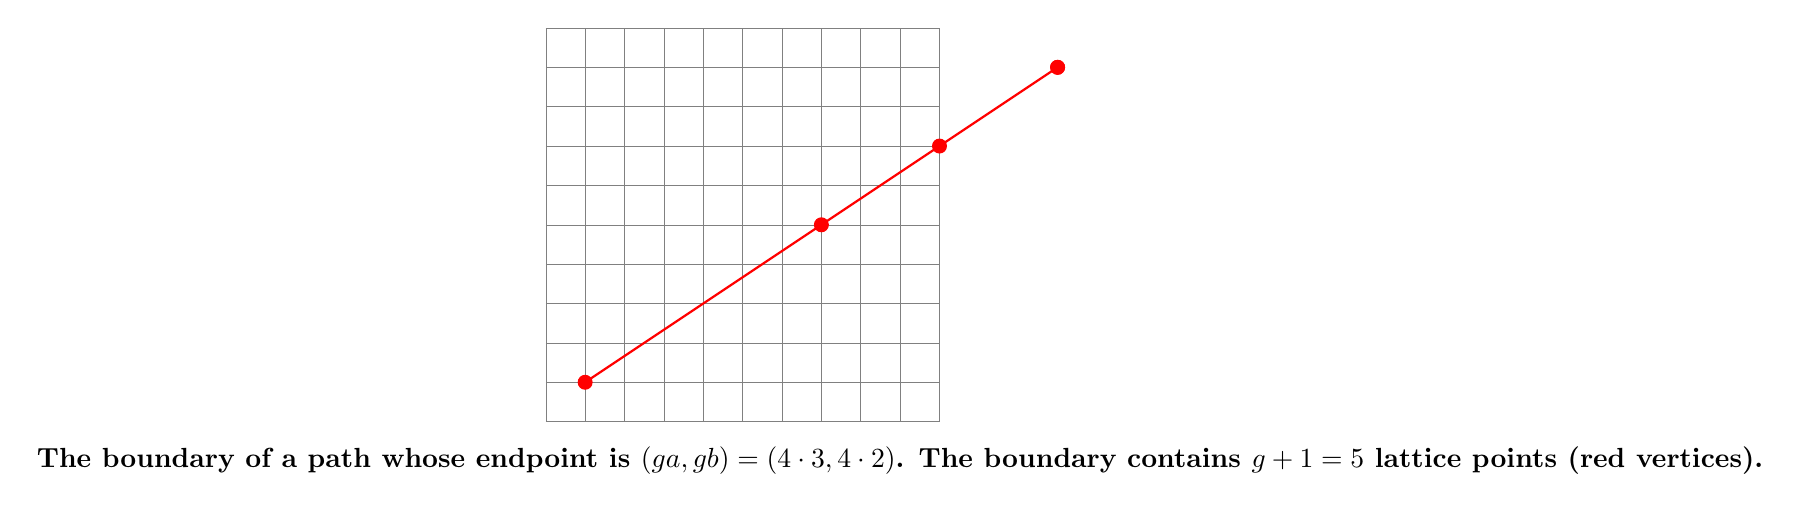
\begin{tikzpicture}[scale=0.5]
    % Draw the grid
    \draw[help lines] (-1,-1) grid (9,9);
    
    % Define the coordinates of the vertices
    \coordinate (A) at (0,0);
    \coordinate (B) at (4*3, 4*2);
    \coordinate (C) at (2*3, 2*2);
    \coordinate (D) at (3*3, 3*2);
    \coordinate (E) at (4*3, 4*2);
    
    % Draw the line connecting the vertices
    \draw[thick, red] (A) -- (B) -- (C) -- (D) -- (E);
    
    % Draw the red vertices as circles
    \filldraw[red] (A) circle (5pt);
    \filldraw[red] (B) circle (5pt);
    \filldraw[red] (C) circle (5pt);
    \filldraw[red] (D) circle (5pt);
    \filldraw[red] (E) circle (5pt);
    
    % Add the caption
    \node at (8, -2) {\textbf{The boundary of a path whose endpoint is $(ga, gb) = (4 \cdot 3, 4 \cdot 2)$. The boundary contains $g + 1 = 5$ lattice points (red vertices).}};
\end{tikzpicture}

\end{document}